%/*******************************************************************************
% * Copyright (c) 2009, medshare GmbH
% * All rights reserved. This program may not be distributed
% * or modified without prior written consent
% *
% * Contributors:
% *    T. Schaller - initial implementation
% *
% *******************************************************************************/
\documentclass[a4paper]{scrartcl}
\usepackage{german}
\usepackage[utf8]{inputenc}
\usepackage{makeidx}
\usepackage{wrapfig}
\makeindex

\usepackage[pdftex]{graphicx}
\DeclareGraphicsExtensions{.pdf,.jpg,.png}

\usepackage{floatflt}
\usepackage[]{hyperref}
\usepackage{color}
\title{Elexis - Afinion AS100 Connector}
\author{medshare GmbH}

\begin{document}

\maketitle
	\begin{center}
		
\includegraphics{elexis_logo}
	\end{center}
	\begin{center}
		
\includegraphics{axis-shield_logo}
	\end{center}
	\begin{center}
		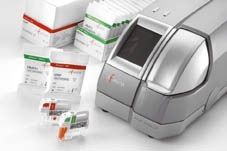
\includegraphics{afinion_device}
	\end{center}
	\begin{center}
		
\includegraphics{afinion_logo}
	\end{center}
\pagebreak

\section{Einf\"uhrung}
Dieses Plugin dient dazu, das Laborger\"at 'Afinion AS100 Analyzer'\footnote{Firma Axis-Shield} an Elexis anzubinden. Mit diesem Plugin k\"onnen die vom Afinion gemessenen Laborparameter direkt in die Elexis-Datenbank eingelesen werden.

\subsection{Voraussetzungen}
Dieses Plugin ben\"otigt Elexis V1.4.0 oder h\"oher sowie einen Afinion AS100 Analyzer Ger\"at. Ausserdem wird ein PC mit mindestens einer freien seriellen Schnittstelle (Alternative: USB To RS-232 Adapter) und ein korrekt gerade verdrahtetes serielles Kabel (kein Nullmodemkabel) zur Verbindung des Afinion mit dem PC ben\"otigt.

\section{Installation und Konfiguration}
Installieren Sie auf dem im Labor befindlichen PC das Plugin wie gewohnt. Verbinden Sie dann bei \textbf{ausgeschalteten} Ger\"aten den Afinion mit der einem seriellen Port des Computers. 
\subsection{Daten\"ubertragungskonfiguration Afinion}
Die serielle Datenkommunikation ist im Afinion standardm\"assig aktiv. Das Ger\"at erfordert zwingend folgende Einstellungen:\\
Baudrate: 115200\\
Daten-Bits: 8\\
Parit\"at: Nein\\
Stop-Bits: 1
\subsection{Elexis Konfiguration}
Starten Sie dann Elexis und gehen Sie dort zu \textsc{Datei-Einstellungen-Datenaustausch- Afinion AS100 Analyzer} (S. Abb. \ref{fig:config}).
\begin{figure}[h]
    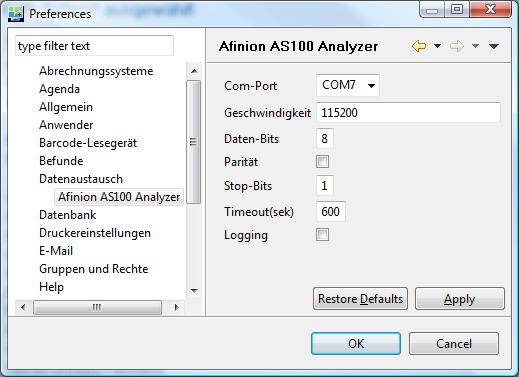
\includegraphics{config}
    \caption{Einstellungen Afinion AS100 Analyzer}
    \label{fig:config}
\end{figure}
Hier stellen Sie den seriellen Port und die Schnittstellenparameter ein. Die Werte m\"ussen mit den Einstellungen auf dem Afinion Ger\"at \"ubereinstimmen (siehe oben). Wichtig: Nach dem \"Andern dieser Parameter m\"ussen Sie Elexis neu starten.

\section{Verwendung}
\begin{figure}[h]
    
\includegraphics{toolbarbutton}
    \caption{Afinion AS100 Analyzer Daten einlesen}
    \label{fig:toolbarbutton}
\end{figure}
Wenn das Plugin korrekt installiert ist, erscheint in der Labor-View automatisch ein neuer Toolbar Button 'Afinion AS100 Analyzer' (Abb. \ref{fig:toolbarbutton}).\\
\\
Ablauf: \\
1. Probenmessung mit dem Afinion durchf\"uhren\\
2. Messwert auf dem Afinion quittieren\\
3. Erst dann den Toolbar Button klicken um die Verbindung mit dem Ger\"at herzustellen.\\
4. Das Abrufen des Messwertes dauert relativ lange (1-2 Minuten).\\
\\
%\begin{figure}[h]
%    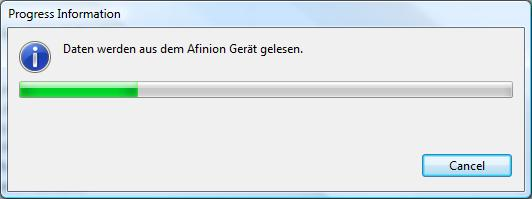
\includegraphics{connected}
%    \caption{Verbindung zum Afinion ist aufgebaut}
%    \label{fig:connected}
%\end{figure}
TODO.\\
%\begin{figure}[h]
%    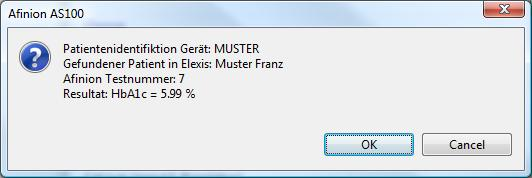
\includegraphics{messwert}
%    \caption{Messwert vom Afinion eingetroffen}
%    \label{fig:messwert}
%\end{figure}
Wenn Elexis ein Resultat empf\"angt, muss dieses einem Patienten zugeordnet werden. Deshalb folgt das Fenster mit der Patientenselektion.\\
\\
\section{Plattformen}
Dieses Plugin wurde unter Windows XP und Vista getestet. Beachten Sie bitte, dass unter Linux die seriellen Ports nicht COM1 usw., sondern /dev/ttyS0 usw. heissen.

\section{Kabelspezifikation}
Es wird ein normales serielles Kabel ben\"otigt (kein Nulllmodemkabel!). Das Kabel muss vom 9-poligen Stecker (m\"annlich) auf den 9-poligen Stecker (weiblich) 1:1 verdrahtet sein. Folgende Pins werden verwendet: 2 (Receive), 3 (Transmit), 5 (Signal GND).\\

\end{document}
